%%
%% forked from https://gits-15.sys.kth.se/giampi/kthlatex kthlatex-0.2rc4 on 2020-02-13
%% expanded upon by Gerald Q. Maguire Jr.
%% This template has been adapted by Anders Sjögren to the University
%% Engineering Program in Computer Science at KTH ICT. Adaptation is the
%% translation of English headings into Swedish as the addition of Swedish
%% text. Original body text is deliberately left in English.


%% Conventions for todo notes:
% \todo[inline]{Comments/directions/... in English}
% \todo[inline, backgroundcolor=kth-lightblue]{Text på svenska}
% \todo[inline, backgroundcolor=kth-lightgreen]{English descriptions about formatting}

%% The template is designed to handle a thesis in English or Swedish
% set the default language to english or swedish by passing an option to the documentclass - this handles the inside tile page
% To optimize for digital output (this changes the color palette add the option: digitaloutput
% To use bibtex or biblatex - include one of these as an option
% For a licentiate thesis or a doctoral dissertation - select g5paper for the booklet format

\documentclass[english, g5paper, bibtex]{kththesis}
%\documentclass[swedish, g5paper, biblatex]{kththesis}

\ifbiblatex
    \usepackage[bibstyle=authoryear,citestyle=authoryear, maxbibnames=99,language=english]{biblatex}
    \addbibresource{references.bib}
    %\DeclareLanguageMapping{norsk}{norwegian}
\else
    % The line(s) below are for BibTeX
    \bibliographystyle{bibstyle/myIEEEtran}
    %\bibliographystyle{apalike}
\fi

%%%%%%%%%%%%%%%%%%%%%%%%%%%%%% Packages %%%%%%%%%%%%%%%%%%%%%%%%%%%%%%
%% The following are needed for generating the DiVA page(s)
\usepackage{scontents}              %% Needed to save lang, abstract, and keywords
\usepackage{pgffor}                 %% includes the foreach loop

%% Basic packages

%% Links
\usepackage{url}                %% Support for breaking URLs

%% Colorize
%\usepackage{color}
\PassOptionsToPackage{dvipsnames, svgnames}{xcolor}

%% Various useful packages
\usepackage[normalem]{ulem}
\usepackage{soul}
\usepackage{xspace}
\usepackage{braket}

% to support units and decimal aligned columns in tables
% the option loads the binary prefixes
\usepackage[binary-units=true, locale=US]{siunitx}

\usepackage{balance}
\usepackage{stmaryrd}
\usepackage{booktabs}
\usepackage{graphicx}	        %% Support for images
\usepackage{multirow}	        %% Support for multirow columns in tables
\usepackage{tabularx}		%% For simple table stretching
\usepackage{mathtools}
\usepackage{algorithm} 
\usepackage{algorithmic}  
\usepackage{amsmath}
\usepackage[linesnumbered,ruled,vlined,algo2e]{algorithm2e}
% can't use both algpseudocode and algorithmic packages
%\usepackage[noend]{algpseudocode}
%\usepackage{subfig}  %% cannot use both subcaption and subfig packages
\usepackage{optidef}
\usepackage{float}		%% Suppor for more flexible floating box positioning
\usepackage{pifont}

%% some additional useful packages
\usepackage{rotating}	    	%% For text rotating
\usepackage{array}		%% For table wrapping
\usepackage{mdwlist}            %% various list-related commands
\usepackage{setspace}           %% For fine-grained control over line spacing

\usepackage{enumitem}           %% to allow changes to the margins of descriptions


%% If you are going to include source code (or code snippets)
\usepackage{listings}		    %% For source code listing
%%\usepackage[cache=false]{minted} %% For source code highlighting
%%\usemintedstyle{borland}

\usepackage{bytefield}          %% For packet drawings
%%----------------------------------------------------------------------------
%%   pcap2tex stuff
%%----------------------------------------------------------------------------
\usepackage{tikz}
\usetikzlibrary{arrows,decorations.pathmorphing,backgrounds,fit,positioning,calc,shapes}
\usepackage{pgfmath}	% --math engine
%\usepackage{xcolor}


\newcommand\bmmax{2}
\usepackage{bm} % bold math

\setlength{\marginparwidth }{4cm} %% needs to be set before the todnotes package is loaded
\usepackage{todonotes}

%% If you are going to include source code (or code snippets)
\usepackage{listings}		%% For source code listing
%%\usepackage[cache=false]{minted} %% For source code highlighting
%%\usemintedstyle{borland}

\usepackage{dirtytalk}

\usepackage{hyperref}
\usepackage[all]{hypcap}	%% prevents an issue related to hyperref and caption linking
%% setup hyperref to use the darkblue color on links
\hypersetup{colorlinks,breaklinks,
            linkcolor=darkblue,urlcolor=darkblue,
            anchorcolor=darkblue,citecolor=darkblue}

\usepackage{notoccite} % do not number captions based on their appearance in the TOC

% to enable rotated figures
\usepackage{rotating}		%% For text rotating

% to allow changes to the margins of descriptions
\usepackage{enumitem}

% Footnotes
\usepackage{perpage}
\usepackage[perpage,para,symbol]{footmisc} %% use symbols to ``number'' footnotes and reset which symbol is used first on each page


%% Managing titles
% \usepackage[outermarks]{titlesec}
%%%%%%%%%%%%%%%%%%%%%%%%%%%%%%%%%%%%%%%%%%%%%%%%%%%%%%%%%%%%%%%%%%%%%%
%\captionsetup[subfloat]{listofformat=parens}

% to include PDF pages
%\usepackage{pdfpages}



\usepackage{csquotes} % Recommended by biblatex

% to provide a float barrier use:
\usepackage{placeins}

%\usepackage{filecontents}          % to be able to store and write to a file) specific contents

\usepackage{comment}  %% Provides a comment environment

\usepackage{kthpaper}

%%% Local Variables:
%%% mode: latex
%%% TeX-master: t
%%% End:
% KTH colors for LaTeX documents
%
% Started from kthcolors by:
% Riccardo Sven Risuleo
% 2016-09-06 11:05:40
%
% from https://github.com/KTH-AC/kthcolors
%
% Adapted using the colors from "Graphic Profile Manual KTH" version 180604
% (i.e.. 2018-06-04) 
% see https://intra.kth.se/en/administration/kommunikation/grafiskprofil/kth-s-grafiska-profil-1.844676
% 
% G. Q. Maguire Jr.
% 2021-07-05
%

%\NeedsTexFormat{LaTeX2e}[1994/06/01]
%\ProvidesPackage{kthcolors}[2021/07/85 v3 Latex package with official KTH colors]

\RequirePackage{xcolor}
%% Primary colors
%% As of the new manual, there is only 1 primary color; but with three 
\definecolor{kth-blue}{RGB/cmyk}{25,84,166/0.849,0.494,0,0.349}
\colorlet{kth-blue80}{kth-blue!80!}
\colorlet{kth-blue40}{kth-blue!40!}

% these are no longer used as of 2018-06-04
%\definecolor{kth-red}{RGB/cmyk}{157,16,45/0,0.898,0.713,0.384}
%\definecolor{kth-green}{RGB/cmyk}{98,146,46/0.329,0,0.685,0.427}

%% Secondary colors
\definecolor{kth-lightblue}{RGB/cmyk}{36,160,216/0.833,0.259,0,0.153}
\colorlet{kth-lightblue80}{kth-lightblue!80!}
\colorlet{kth-lightblue40}{kth-lightblue!40!}

%\definecolor{kth-lightred}{RGB/cmyk}{228,54,62/0,0.763,0.728,0.106}
\definecolor{kth-lightred}{RGB}{216,84,151}
\colorlet{kth-lightred80}{kth-lightred!80!}
\colorlet{kth-lightred40}{kth-lightred!40!}

\definecolor{kth-lightgreen}{RGB/cmyk}{176,201,43/0.124,0,0.786,0.212} % olive
\colorlet{kth-lightgreen80}{kth-lightgreen!80!}
\colorlet{kth-lightgreen40}{kth-lightgreen!40!}

% Cool Gray 9C
%\definecolor{kth-coolgray}{RGB}{101,101,108}

% Cool Gray 10 suggested by Martin Krzywinski (see http://mkweb.bcgsc.ca/colorblind) 
\definecolor{kth-coolgray}{RGB}{99,102,106}
\colorlet{kth-coolgray80}{kth-coolgray!80!}
\colorlet{kth-coolgray40}{kth-coolgray!40!}

% Tertiary colors (yet more colors)
% All of these are no longer used
%\definecolor{kth-pink}{RGB/cmyk}{216,84,151/10,0.611,0.301,0.153}
%\definecolor{kth-yellow}{RGB/cmyk}{250,185,25/0,0.26,0.9,0.0196}
%\definecolor{kth-darkgray}{RGB/cmyk}{101,101,108/0.0648,0.0648,0,0.576}
%\definecolor{kth-middlegray}{RGB/cmyk}{189,188,188/0,0.00529,0.00529,0.259}
%\definecolor{kth-lightgray}{RGB/cmyk}{227,229,227/0.00873,0,0.00873,0.102}

%\DeclareOption{gray}{\colorlet{gray}{kth-darkgray}}

% These versions are designed to meet accessability requirements for digital media
% Note that the palette is more limited than for the print version of the colors
\ifdigitaloutput
    % primary color
    \definecolor{kth-blue}{HTML}{1954A6} % Deep sea
    \definecolor{kth-blue80}{HTML}{5E87C0}

    % Secondary colors
    \definecolor{kth-lightblue}{HTML}{2191C4} % Stratosphere
    \definecolor{kth-lightred}{HTML}{D02F80} % Fluorescence
    \definecolor{kth-lightred80}{HTML}{D95599}
    \definecolor{kth-lightgreen}{HTML}{62922E} % Front-lawn
    \definecolor{kth-coolgray}{HTML}{65656C} % Office
    \definecolor{kth-coolgray80}{HTML}{848489}
\fi



%%% custom definitions
%% Coloring the links!
\newcommand\myshade{75} % Usage: red!\myshade!black

\definecolor{ForestGreen} {RGB}{34,  139,  34}
\definecolor{HeraldRed2}   {rgb}{0.81, 0.12, 0.15}

\newcommand{\refscolor} {blue}
\newcommand{\linkscolor}{HeraldRed2}
\newcommand{\urlscolor} {ForestGreen}

\newcommand{\smartparagraph}[1]{\vspace{.05in}\noindent\textbf{#1}}

\hypersetup{
	colorlinks  = true,
	breaklinks  = true,
	linkcolor   = \linkscolor,
	urlcolor    = \urlscolor,
	citecolor   = \refscolor,
	anchorcolor = black
}


%% My custom commands
%\newcommand*{\eg}{e.g.,\@\xspace}
%\newcommand*{\ie}{i.e.,\@\xspace}
%\newcommand*{\etc}{etc.\@\xspace}
%\newcommand*{\etal}{et al.\@\xspace}
%\newcommand*{\addthinspace}{\hskip0.16667em\relax}

\def\first {$(i)$\xspace}
\def\second{$(ii)$\xspace}
\def\third {$(iii)$\xspace}
\def\fourth{$(iv)$\xspace}
\def\fifth {$(v)$\xspace}
\def\sixth {$(vi)$\xspace}

%% Footnotes with symbols
\renewcommand{\thefootnote}{\fnsymbol{footnote}}
\if 0
	\renewcommand{\thefootnote}{\arabic{footnote}}
\fi
\setlength{\skip\footins}{0.23cm}

%% Limit hyphenation
\hyphenpenalty=9000
\tolerance=5000

%% ToC depth 
\setcounter{secnumdepth}{4} % how many sectioning levels to assign numbers to
\setcounter{tocdepth}{4}    % how many sectioning levels to show in ToC

\makeatletter
\newcommand{\DeclareLatinAbbrev}[2]{%
  \DeclareRobustCommand{#1}{%
    \@ifnextchar{.}{\textit{#2}}{%
      \@ifnextchar{,}{\textit{#2.}}{%
        \@ifnextchar{!}{\textit{#2.}}{%
          \@ifnextchar{?}{\textit{#2.}}{%
            \@ifnextchar{)}{\textit{#2.}}{%
              {\textit{#2.,\ }}}}}}}}%
}
\makeatother
\DeclareLatinAbbrev{\eg}{e.g}
\DeclareLatinAbbrev{\Eg}{E.g}
\DeclareLatinAbbrev{\ie}{i.e}
\DeclareLatinAbbrev{\Ie}{I.e}
\DeclareLatinAbbrev{\etc}{etc}
\DeclareLatinAbbrev{\etal}{et~al}

\newcommand*{\todoinline}[1]{\textcolor{red}{TODO: #1}}  % load some additional definitions to make writing more consistent

% The following is needed in conjunction with generating the DiVA data with abstracts and keywords using the scontents package and a modified listings environment
%\usepackage{listings}   %  already included
\ExplSyntaxOn
\newcommand\typestoredx[2]{\expandafter\__scontents_typestored_internal:nn\expandafter{#1} {#2}}
\ExplSyntaxOff
\makeatletter
\let\verbatimsc\@undefined
\let\endverbatimsc\@undefined
\lst@AddToHook{Init}{\hyphenpenalty=50\relax}
\makeatother

\lstnewenvironment{verbatimsc}
    {
    \lstset{%
        basicstyle=\ttfamily\tiny,
        %basicstyle=\tiny,
        %columns=fullflexible,
        columns=[l]fixed,
        language=[LaTeX]TeX,
        %numbers=left,
        %numberstyle=\tiny\color{gray},
        keywordstyle=\color{red},
        breaklines=true,                 % sets automatic line breaking
        breakatwhitespace=true,          % sets if automatic breaks should only happen at whitespace
        %keepspaces=false,
        breakindent=0em,
        %fancyvrb=true
    }
}{}

%% Reduce hyphenation as much as possible
\hyphenpenalty=15000 
\tolerance=1000

%% definition of new command for bytefield package
\newcommand{\colorbitbox}[3]{%
	\rlap{\bitbox{#2}{\color{#1}\rule{\width}{\height}}}%
	\bitbox{#2}{#3}}

% to find unicode characters that LaTeX complains about
%\DeclareUnicodeCharacter{F0DE}{XXXX Here I am?????XXXX}

% packages that have to be included after hyperref
\usepackage{doi}
\usepackage{cleveref}           %% Replace Section with a symbol


%% Acronyms
%\usepackage[acronym]{polyglossia}
%\usepackage[acronym]{glossaries}
\usepackage[acronym, section=section, nonumberlist, nomain, nopostdot]{glossaries}

%% Acronyms
% note that nonumberlist - removes the cross references to the pages where the acronym appears
% note that nomain - does not produce a main gloassay, this only acronyms will be in the glossary
% note that nopostdot - will present there being a period at the end of each entry
\ifinswedish
    %\usepackage{glossaries-swedish}
\fi
%\glsdisablehyper
\makeglossaries
%%% Local Variables:
%%% mode: latex
%%% TeX-master: t
%%% End:

% note the use of a non-breaking dash in long text for the following acronym
\newacronym{IQL}{IQL}{Independent Q‑Learning}

\newacronym{LAN}{LAN}{Local Area Network}
\newacronym{SDG}{SDG}{Sustainable Development Goal}

% note the use of a non-breaking dash in the following acronym
\newacronym{WiFi}{Wi-Fi}{Wireless Fidelity}

\newacronym{WLAN}{WLAN}{Wireless Local Area Network}
\newacronym{UN}{UN}{United Nations}

                %load the acronyms file



\begin{document}
%% if using XeLaTex uncomment the following
%\selectlanguage[variant=american]{english}
%% otherwise
%\selectlanguage{UKenglish}
%\selectlanguage{english}


%% Information for inside title page
\ifinswedish
  \selectlanguage{swedish}
  \title{Titeln på avhandlingens språk}
  \subtitle{En undertiteln på avhandlingens språk}
%You: Note that the commands you are using are for biblatex and not bibtex. So you have to change the include files to include biblatex also you have to change the way that the reference bib file is included.

  \alttitle{English translation of the title}
  \altsubtitle{English translation of the subtitle}
\else
   \selectlanguage{english}
   \title{The title in the language of the thesis}
   \subtitle{A subtitle in the language of the thesis}
    % give the alternative title - i.e., if the thesis is in English, then give a Swedish title
   \alttitle{Detta är den svenska översättningen av titeln}
   \altsubtitle{Detta är den svenska översättningen av undertiteln}
% alternative, if the thesis is in Swedish, then give an English title

\fi

%%% Uncomment the program that you are in
%\programcode{KTHARK}% Architecture
%\programcode{KTHBIO}% Biotechnology
%\programcode{KTHBYV}% Civil and Architectural Engineering
\programcode{KTHDAT}% Computer Science
%\programcode{KTHEST}% Electrical Engineerin
%\programcode{KTHEGI}% Energy Technology and Systems
%\programcode{KTHFTK}% Vehicle and Maritime Engineering
%\programcode{KTHFYS}% Physics
%\programcode{KTHGEO}% Geodesy and Geoinformatics
%\programcode{KTHHFL}% Solid Mechanics
%\programcode{KTHIEO}% Industrial Economics and Management
%\programcode{KTHIIP}% Production Engineering
%\programcode{KTHIKT}% Information and Communication Technology
%\programcode{KTHKEV}% Chemical Science and Engineering
%\programcode{KTHKON}% Art, Technology and Design
%\programcode{KTHMAT}% Mathematics
%\programcode{KTHKOM}% Mediated Communication
%\programcode{KTHPBA}% Planning and Decision Analysis
%\programcode{KTHSHB}% The Built Environment and Society: Management, Economics and Law
%\programcode{KTHTMV}% Engineering Materials Science
%\programcode{KTHMEK}% Engineering Mechanics
%\programcode{KTHTKB}% Theoretical Chemistry and Biology

%% Alternatively, you can say \programme{xx} to directly set the programme string

%\schoolAcronym{ABE}
%\schoolAcronym{CBH}
\schoolAcronym{EECS}
%\schoolAcronym{ITM}
%\schoolAcronym{SCI}
%% Alternatively, you can say \school{School of xx} to directly set the school string

\authorsLastname{Student}
\authorsFirstname{Oscar}
\email{oscars@kth.se}
\kthid{u1xxxxxx}
\orcid{0000-0002-0007-746X}
\authorsDepartment{Computer Science}

\ifinswedish
    \examen{doktorsexamen}
    %\examen{Ekonomie doktorsexamen}
\else
    \examen{Doctor of Technology}
    %\examen{Doctor of Philosophy}
\fi

\ifinswedish
    \thesistype{Doktorsavhandling}
\else
    \thesistype{Doctoral Thesis}
\fi

\ifinswedish
    \disputationsdatum{Måndag den 15 Mars 2021 klockan 13:00 CET}
\else
    \disputationsdatum{Monday the 15\textsuperscript{th} March 2021 at 13:00 CET}
\fi

\ifinswedish
    \disputationslokal{ett Zoom-Webinar}
\else
    \disputationslokal{via Zoom}
\fi

%	"Room": "Seminar room Grimeton at COM",
%	"Address": "Kistagången 16, East, Floor 4, Elevator B",
%	"City": "Kista"

\presentationDateAndTimeISO{2021-03-15 13:00}
\presentationLanguage{eng}
\presentationRoom{via Zoom}
%\presentationAddress{}
\presentationCity{Stockholm}

\isbn{ISBN 978-91-7873-xxx-y}
\trita{TRITA-ITM-AVL 2021:x}
\publisher{Universitetsservice US AB}

\publicationYear{\the\year{}}
\publicationMonth{\the\month{}}

%% Supervisors' information
% first supervisor (A)
\supervisorAsLastname{Maguire Jr.}
\supervisorAsFirstname{Gerald Q.}
\supervisorAsEmail{maguire@kth.se}
% if not with KTH then enter the name of the external organization
%\supervisorAsOrganization{University of Nowhere, School of Hard, Department of Knocks}
\supervisorAsKTHID{u1d13i2c}
\supervisorAsSchool{EECS}
\supervisorAsDepartment{Computer Science}
% second supervisor (B)
\supervisorBsLastname{Adviser}
\supervisorBsFirstname{Secondary}
\supervisorBsEmail{secondary.adviser@foo.edu}
% if not with KTH then enter the name of the external organization
\supervisorBsOrganization{University of Nowhere, School of Hard, Department of Knocks}
% otherwise, enter the supervisor's KTHID, KTH School and Department information
%\supervisorBsKTHID{u10000c}
%\supervisorBsSchool{School of xxx}
%\supervisorBsDepartment{dept}

% Opponent's information
\opponentsLastname{Normal}
\opponentsFirstname{A. B.}
\opponentsEmail{ABNormal@example.org}
% for an opponent outside KTH define:
\opponentsOrganization{Famous Anvils}
% for an opponent inside KTH define:
%\opponentsSchool{Circus school}
%\opponentsDepartment{Clown department}

%%%%% for DiVA's National Subject Category information
%%% Enter one or more 3 or 5 digit codes
%%% See https://www.scb.se/contentassets/3a12f556522d4bdc887c4838a37c7ec7/standard-for-svensk-indelning--av-forskningsamnen-2011-uppdaterad-aug-2016.pdf
%%% See https://www.scb.se/contentassets/10054f2ef27c437884e8cde0d38b9cc4/oversattningsnyckel-forskningsamnen.pdf
%%%%
%%%% Some examples of these codes are shown below:
% 102 Data- och informationsvetenskap (Datateknik)    Computer and Information Sciences
% 10201 Datavetenskap (datalogi) Computer Sciences 
% 10202 Systemvetenskap, informationssystem och informatik (samhällsvetenskaplig inriktning under 50804)
% Information Systems (Social aspects to be 50804)
% 10203 Bioinformatik (beräkningsbiologi) (tillämpningar under 10610)
% Bioinformatics (Computational Biology) (applications to be 10610)
% 10204 Människa-datorinteraktion (interaktionsdesign) (Samhällsvetenskapliga aspekter under 50803) Human Computer Interaction (Social aspects to be 50803)
% 10205 Programvaruteknik Software Engineering
% 10206 Datorteknik Computer Engineering
% 10207 Datorseende och robotik (autonoma system) Computer Vision and Robotics (Autonomous Systems)
% 10208 Språkteknologi (språkvetenskaplig databehandling) Language Technology (Computational Linguistics)
% 10209 Medieteknik Media and Communication Technology
% 10299 Annan data- och informationsvetenskap Other Computer and Information Science
%%%
% 202 Elektroteknik och elektronik Electrical Engineering, Electronic Engineering, Information Engineering
% 20201 Robotteknik och automation Robotics
% 20202 Reglerteknik Control Engineering
% 20203 Kommunikationssystem Communication Systems
% 20204 Telekommunikation Telecommunications
% 20205 Signalbehandling Signal Processing
% 20206 Datorsystem Computer Systems
% 20207 Inbäddad systemteknik Embedded Systems
% 20299 Annan elektroteknik och elektronik Other Electrical Engineering, Electronic Engineering, Information Engineering
%% Example for a thesis in Computer Science and Computer Systems
\nationalsubjectcategories{10201, 10206}

% Enter the English and Swedish keywords here for use in the PDF meta data _and_ for later use
% following the respective abstract.
% Try to put the words in the same order in both to facilitate matching.
\EnglishKeywords{Canvas Learning Management System, Docker containers, Performance tuning}
\SwedishKeywords{Canvas Lärplattform, Dockerbehållare, Prestandajustering}

% Put the title, author, and keyword information into the PDF meta information
% This file contains the LaTeX to add information to the PDF file (specifically, author(s), title(s), and keywords
% It uses the hyperref package and should be be included before the \begin{document}
%
% I want to acknowledge the inspiration of Karl Voit's template for TU Graz that inspired me to add the PDF document information
% For more information about his template see https://github.com/novoid/LaTeX-KOMA-template
% Note that this template does not use anything from his template other than the names of the information for the PDF meta fields, i.e., mytitle, myauthor, and mykeywords together with the idea of defining the corresponding newcommand to set the relevant hyperref parameters.

\makeatletter
\ifx\@subtitle\@empty
    \newcommand{\mytitle}{\@title}
\else
    \newcommand{\mytitle}{\@title: \@subtitle}
\fi
\makeatother

\hypersetup{
     pdftitle={\mytitle}        % Title field
}

\makeatletter
\newcommand{\myauthor}{\@authorsFirstname\space\@authorsLastname} 
\makeatother

\hypersetup{
     pdfauthor={\myauthor}      % Author field
}

% Put the alternative title (and subtitle) into the PDF Subject meta
\makeatletter
\ifx\@altsubtitle\@empty\relax
    \newcommand{\myalttitle}{\@alttitle}
\else
    \newcommand{\myalttitle}{\@alttitle: \@altsubtitle}
\fi
\makeatother

\hypersetup{
     pdfsubject={\myalttitle}        % Subject field
}

\makeatletter
\ifx\@EnglishKeywords\@empty
    \ifx\@SwedishKeywords\@empty
        \newcommand{\mykeywords}{}
    \else
    \newcommand{\mykeywords}{\@SwedishKeywords}
    \fi
\else
    \ifx\@SwedishKeywords\@empty
        \newcommand{\mykeywords}{\@EnglishKeywords}
    \else
        \ifinswedish
            \newcommand{\mykeywords}{\@SwedishKeywords, \@EnglishKeywords}
        \else
            \newcommand{\mykeywords}{\@EnglishKeywords, \@SwedishKeywords}
        \fi
    \fi
\fi
\makeatother

\hypersetup{
     pdfkeywords={\mykeywords}        % Keywords field
}        
% I have _not_ set the following fields:
%    pdfcreator             % Creator field
%    pdfproducer            % Producer field
 

\titlepage
% document/book information page
\bookinfopage

% Frontmatter includes the abstracts and table-of-contents
\frontmatter
\setcounter{page}{1}

\begin{abstract}
% The first abstract should be in the language of the thesis.
% Abstract fungerar på svenska också.
  \markboth{\abstractname}{}
\begin{scontents}[store-env=lang]
eng
\end{scontents}
%%% The contents of the abstract will be saved in LaTeX format and output on the page(s) at the end of the thesis with information for DiVA facilitating the correct entry of the meta data for your thesis. These page(s) will be removed before the thesis is to be inserted into DiVA.
\begin{scontents}[store-env=abstracts,print-env=true]
\todo[inline, backgroundcolor=kth-lightgreen]{All theses at KTH are \textbf{required} to have an abstract in both \textit{English} and \textit{Swedish}.}

\todo[inline, backgroundcolor=kth-lightgreen]{Keep in mind that most of your potential readers are only going to read your \texttt{title} and \texttt{abstract}. This is why it is important that the abstract give them enough information that they can decide is this document relevant to them or not. Otherwise the likely default choice is to ignore the rest of your document.\\

A abstract should stand on its own, i.e., no citations, cross references to the body of the document, acronyms must be spelled out, \ldots .\\

Write this early and revise as necessary. This will help keep you focused on what you are trying to do.}

Write an abstract that is about 250 and 350 words (1/2 A4-page)  with the following components:
\begin{itemize}
  \item What is the topic area? (optional) Introduces the subject area for the project.
  \item Short problem statement
  \item Why was this problem worth a third cycle thesis/dissertation? (\ie, why is the problem both significant and of a suitable degree of difficulty for the degree? Why has no one else solved it yet?)
  \item How did you solve the problem? What was your method/insight?
  \item Results/Conclusions/Consequences/Impact: What are your key results and conclusions? What will others do based upon your results? What can be done now that you have finished - that could not be done before your thesis project was completed?
  \textbf{The presentation of the results should be the main part of the abstract.}
\end{itemize}
\end{scontents}

\subsection*{Keywords}
\begin{scontents}[store-env=keywords,print-env=true]
5-6 keywords\\
% If you set the EnglishKeywords earlier, you can retrieve them with:
% Alternative 1:
%\makeatletter
%\@EnglishKeywords
%\makeatother
%
% Alternative 2:
\InsertKeywords{english}
% If you did not set the EnglishKeywords earlier then simply enter the keywords here:
% Alternative 3:
% comma separate keywords, such as: Canvas Learning Management System, Docker containers, performance tuning

\todo[inline, backgroundcolor=kth-lightgreen]{\textbf{Choosing good keywords can help others to locate your paper, thesis, dissertation, \ldots and related work.}}
Choose the most specific keyword from those used in your domain, see for example: the ACM Computing Classification System ({\small \url{https://www.acm.org/publications/computing-classification-system/how-to-use})},
the IEEE Taxonomy ({\small \url{https://www.ieee.org/publications/services/thesaurus-thank-you.html}}), PhySH (Physics Subject Headings)\linebreak[4] ({\small \url{https://physh.aps.org/}}), \ldots or keyword selection tools such as the  National Library of Medicine's Medical Subject Headings (MeSH)  ({\small \url{https://www.nlm.nih.gov/mesh/authors.html}}) or Google's Keyword Tool ({\small \url{https://keywordtool.io/}})\\

\textbf{Mechanics}:
\begin{itemize}
  \item The first letter of a keyword should be set with a capital letter and proper names should be capitalized as usual.
  \item Spell out acronyms and abbreviations.
  \item Avoid "stop words" - as they generally carry little or no information.
  \item List your keywords separated by commas (",").
\end{itemize}    
Since you should have both English and Swedish keywords - you might think of ordering them in corresponding order (\ie, so that the n\textsuperscript{th} word in each list correspond) - this makes it easier to mechanically find matching keywords.

\end{scontents}
\end{abstract}

\cleardoublepage
\babelpolyLangStart{swedish}
  \begin{abstract}
    \markboth{\abstractname}{}
\begin{scontents}[store-env=lang]
swe
\end{scontents}
\begin{scontents}[store-env=abstracts,print-env=true]
\todo[inline, backgroundcolor=kth-lightblue]{Alla avhandlingar vid KTH \textbf{måste ha} ett abstrakt på både \textit{engelska} och \textit{svenska}.\\

Om du skriver din avhandling på svenska ska detta göras först (och placera det som det första abstraktet) - och du bör revidera det vid behov.}

\todo[inline]{If you are writing your thesis in English, you can leave this until the final version. If you are writing your thesis in Swedish then this should be done first – and you should revise as necessary along the way.\\
If you are writing your thesis in English, then this section can be a summary targeted at a more general reader. However, if you are writing your thesis in Swedish, then the reverse is true – your abstract should be for your target audience, while an English summary can be written targeted at a more general audience.\\
This means that the English abstract and Swedish sammnfattning  
or Swedish abstract and English summary need not be literal translations of each other.}

\todo[inline, backgroundcolor=kth-lightgreen]{The abstract in the language used for the thesis should be the first abstract, while the Summary/Sammanfattning in the other language can follow.}

\todo[inline, backgroundcolor=kth-lightgreen]{Exchange students many want to include one or more abstracts in the language(s) used in their home institutions to avoid the neeed to write another thesis when returning to their home institution.}

\end{scontents}
\subsection*{Nyckelord}
\begin{scontents}[store-env=keywords,print-env=true]
5-6 nyckelord\\
% SwedishKeywords were set earlier, hence we can use alternative 2
\InsertKeywords{swedish}
\todo[inline, backgroundcolor=kth-lightblue]{Nyckelord som beskriver innehållet i uppsatsrapporten}
\end{scontents}
\end{abstract}
\babelpolyLangStop{swedish} % Ends language block
\cleardoublepage
\todo[inline, backgroundcolor=kth-lightgreen]{Note that you may need to augment the set of language used in polyglossia or
babel (see the file kththesis.cls). The following languages include those languages that were used in theses at KTH in 2018-2019, except for one in Chinese.\\
Remove those versions that you do not need.\\
If adding a new language, when specifying the language for the abstract use the three letter ISO 639-2 Code – specifically the "B" (bibliographic) variant of these codes (note that this is the same language code used in DiVA).}
\todo[inline]{Use the relevant language for abstracts for your home university.}
\babelpolyLangStart{french} 
\begin{abstract}
    \markboth{\abstractname}{}
\begin{scontents}[store-env=lang]
fre
\end{scontents}
\begin{scontents}[store-env=abstracts,print-env=true]
Résumé en français
\end{scontents}
\subsection*{Mots clés}
\begin{scontents}[store-env=keywords,print-env=true]
5-6 mots-clés
\end{scontents}
\end{abstract}
\babelpolyLangStop{french}
\cleardoublepage
\babelpolyLangStart{spanish}
\begin{abstract}
    \markboth{\abstractname}{}
\begin{scontents}[store-env=lang]
spa
\end{scontents}
\begin{scontents}[store-env=abstracts,print-env=true]
Résumé en espagnol.
\end{scontents}
Résumé en espagnol

\subsection*{Palabras claves}
\begin{scontents}[store-env=keywords,print-env=true]
5-6 Palabras claves
\end{scontents}
\end{abstract}
\babelpolyLangStop{spanish}
\cleardoublepage
\babelpolyLangStart{italian}
\begin{abstract}
    \markboth{\abstractname}{}
\begin{scontents}[store-env=lang]
ita
\end{scontents}
\begin{scontents}[store-env=abstracts,print-env=true]
Sommario in italiano.
\end{scontents}
\subsection*{parole chiave}
\begin{scontents}[store-env=keywords,print-env=true]
5-6 parole chiave
\end{scontents}
\end{abstract}
\babelpolyLangStop{italian}
\cleardoublepage
% note that a macro is used to avoid Overleaf parsing problems
\babelpolyLangStart{norsk}
\begin{abstract}
    \markboth{\abstractname}{}
\begin{scontents}[store-env=lang]
nor
\end{scontents}
\begin{scontents}[store-env=abstracts,print-env=true]
Sammendrag på norsk.
\end{scontents}
\subsection*{Nøkkelord}
\begin{scontents}[store-env=keywords,print-env=true]
5-6 nøkkelord
\end{scontents}
\end{abstract}
\babelpolyLangStop{norsk}
\cleardoublepage
% note that a macro is used to avoid Overleaf parsing problems
\babelpolyLangStart{ngerman}
\begin{abstract}
    \markboth{\abstractname}{}
\begin{scontents}[store-env=lang]
ger
\end{scontents}
\begin{scontents}[store-env=abstracts,print-env=true]
Zusammenfassung in Deutsch.
\end{scontents}
\subsection*{Schlüsselwörter}
\begin{scontents}[store-env=keywords,print-env=true]
5-6 Schlüsselwörter
\end{scontents}
\end{abstract}
\babelpolyLangStop{ngerman}
\cleardoublepage
\babelpolyLangStart{danish}
\begin{abstract}
    \markboth{\abstractname}{}
\begin{scontents}[store-env=lang]
dan
\end{scontents}
\begin{scontents}[store-env=abstracts,print-env=true]
Abstrakt på dansk.
\end{scontents}
\subsection*{Søgeord}
\begin{scontents}[store-env=keywords,print-env=true]
5-6 Søgeord
\end{scontents}
\end{abstract}
\babelpolyLangStop{danish}
\cleardoublepage
\babelpolyLangStart{dutch}
\begin{abstract}
    \markboth{\abstractname}{}
\begin{scontents}[store-env=lang]
dut
\end{scontents}
\begin{scontents}[store-env=abstracts,print-env=true]
Samenvatting in het Nederlands.
\end{scontents}
\subsection*{Trefwoorden}
\begin{scontents}[store-env=keywords,print-env=true]
5-6 trefwoorden
\end{scontents}
\end{abstract}
\babelpolyLangStop{dutch}
\cleardoublepage
\babelpolyLangStart{estonian}
\begin{abstract}
    \markboth{\abstractname}{}
\begin{scontents}[store-env=lang]
est
\end{scontents}
\begin{scontents}[store-env=abstracts,print-env=true]
Eesti keeles kokkuvõte.
\end{scontents}
\subsection*{Märksõnad}
\begin{scontents}[store-env=keywords,print-env=true]
5-6 Märksõnad
\end{scontents}
\end{abstract}
\babelpolyLangStop{estonian}
\cleardoublepage
% set to the language of the body of the thesis

%\selectlanguage{swedish}
\selectlanguage{english}


\section*{Acknowledgments }
\markboth{Acknowledgments}{}
\todo[inline]{It is nice to acknowledge the people that have helped you. It is
  also necessary to acknowledge any special permissions that you have gotten –
  for example getting permission from the copyright owner to reproduce a
  figure. In this case you should acknowledge them and this permission here
  and in the figure’s caption. \\
  Note: If you do not have the copyright owner’s permission, then you cannot use any copyrighted figures/tables/… .
}
\todo[inline, backgroundcolor=kth-lightblue]{I detta kapitel kan du e v nämna något om
  din bakgrund om det påverkar rapporten på något sätt. Har du t ex inte
  möjlighet att skriva perfekt svenska för att du är nyanländ till landet kan
  det vara på sin plats att nämna detta här. OBS, detta får dock inte vara en
  ursäkt för att lämna in en rapport med undermåligt språk, grammatik och
  stavning (t ex får fel som en automatisk stavningskontroll och
  grammatikkontroll kan upptäcka inte förekomma)\\

En dualism som måste hanteras i hela rapporten och projektet
}

I would like to thank xxxx for having yyyy.\\

\acknowlegmentssignature

\fancypagestyle{plain}{}
\renewcommand{\chaptermark}[1]{ \markboth{#1}{}} 
\tableofcontents
  \markboth{\contentsname}{}

\cleardoublepage
\listoffigures

\cleardoublepage

\listoftables
\cleardoublepage
\lstlistoflistings\todo[inline, backgroundcolor=kth-lightgreen]{If you have listings in your thesis, otherwise delete this preface page.}
\cleardoublepage
\printglossary[type=\acronymtype, title={List of acronyms and abbreviations}]
\todo[inline, backgroundcolor=kth-lightgreen]{The list of acronyms and abbreviations should be in alphabetical order based on the spelling of the acronym or abbreviation.
}
\label{pg:lastPageofPreface}
% Mainmatter is where the actual contents of the thesis goes
\mainmatter

\renewcommand{\chaptermark}[1]{\markboth{#1}{}}
\chapter{Introduction}
\label{ch:introduction}
\todo[inline, backgroundcolor=kth-lightblue]{Introduktion}
\todo[inline]{This chapter describes the
specific problem that this thesis addresses, the context of the problem, the
goals of this thesis project, and outlines the structure of the thesis.}
\todo[inline, backgroundcolor=kth-lightgreen]{The first paragraph after a heading is not indented, all of the
  subsequent paragraphs have their first line indented.}

\todo[inline]{Give a general introduction to the area. (Remember to use appropriate references in this and all other sections.)}


% One can use either biblatex or bibtex - set as the option for the document at the top of this file
\ifbiblatex
\todo[inline, backgroundcolor=kth-lightgreen]{We use the \emph{biblatex} package to handle our references.  We
use the command \texttt{parencite} to get a reference in parenthesis, like
this \textbackslash parencite\{heisenberg2015\} resulting in \parencite{heisenberg2015}.  It is also possible to include the author as part of the sentence using \texttt{textcite}, like talking about the work of \textbackslash textcite\{einstein2016\} resulting in \textcite{einstein2016}.\\
This also means that you have to change the include files to include biblatex and change the way that the reference.bib file is included.}
\else
\todo[inline, backgroundcolor=kth-lightgreen]{We use the \emph{bibtex} package to handle our references.  We therefore
use the command \textbackslash cite\{farshin\_make\_2019\}. For example, Farshin, \etal described how to improve LLC
cache performance in \cite{farshin_make_2019} in the context of links running
at \SI{200}{Gbps}.}
\fi

\todo[inline, backgroundcolor=kth-lightgreen]{Use the glossaries package to help yourself and your readers.
Add the acronyms and abbreviations to lib/acronyms.tex. Some examples are shown below:}
In this thesis we will examine the use of \glspl{LAN}. In this thesis we will
assume that \glspl{LAN} include \glspl{WLAN}, such as \gls{WiFi}.

\section{Background}
\label{sec:background}
\todo[inline, backgroundcolor=kth-lightblue]{Bakgrund}
\todo[inline]{Present the background for the area. Set the context for your project – so that your reader can understand both your project and this thesis. (Give detailed background information in Chapter 2 - together with related work.)\\
Sometimes it is useful to insert a system diagram here so that the reader knows what are the different elements and their relationship to each other. This also introduces the names/terms/… that you are going to usethroughout your thesis (be consistent). This figure will also help you later delimit what you are going to do and what others have done or will do.}

As one can find in RFC 1235\,\cite{ioannidis_coherent_1991} multicast is useful for xxxx .



\section{Problem}
\label{sec:problem}
\todo[inline, backgroundcolor=kth-lightblue]{Problemdefinition / Frågeställning}

\todo[inline]{Longer problem statement\\
If possible, end this section with a question as a problem statement.}

% Research Question
%\label{sec:researchQuestion}
\section{Purpose}
\label{sec:purpose}
\todo[inline, backgroundcolor=kth-lightblue]{Syfte}
\todo[inline]{State the purpose  of your thesis and research.

Describe who benefits and how they benefit if you achieve your goals. Include anticipated ethical, sustainability, social issues, \etc related to your project. (Return to these in your reflections in Section~\ref{sec:reflections}.)}

\section{Goals}
\label{sec:goals}
\todo[inline, backgroundcolor=kth-lightblue]{Mål}

\todo[inline]{State the goal/goals of this degree project.

In addition to presenting the goal(s), you might also state what the deliverables and results of the project are.} 

\section{Research Methodology}
\label{sec:researchMethodology}
\todo[inline, backgroundcolor=kth-lightblue]{Forskningsmetodik}

\todo[inline]{Introduce your choice of methodology/methodologies and method/methods – and the reason why you chose them. Contrast them with and explain why you did not choose other methodologies or methods. (The details of the actual methodology and method you have chosen will be given in Chapter~\ref{ch:methods}. Note that in Chapter~\ref{ch:methods}, the focus could be research strategies, data collection, data analysis, and quality assurance.)\\
In this section you should present your philosophical assumption(s), research method(s), and research approach(es).}

\section{Delimitations}
\label{sec:deliminations}
\todo[inline, backgroundcolor=kth-lightblue]{Avgränsningar}
\todo[inline]{Describe the boundary/limits of your thesis project and what you are explicitly not going to do. This will help you bound your efforts – as you have clearly defined what is out of the scope of this thesis project. Explain the delimitations. These are all the things that could affect the study if they were examined and included in the degree project.}

\section{Structure of the thesis}
\todo[inline, backgroundcolor=kth-lightblue]{ Avhandlingens disposition}
Chapter~\ref{ch:background} presents relevant background information about xxx.  Chapter~\ref{ch:methods} presents the methodology and method used to solve the problem. …

\cleardoublepage
\chapter{Background}
\label{ch:background}
\todo[inline, backgroundcolor=kth-lightblue]{Bakgrund}

\todo[inline]{When you do your literature study, you should have a nearly complete Chapters 1 and 2.\\
You may also find it convenient to introduce the future work section into your report early – so that you can put things that you think about but decide not to do now into this section.\\
Note that later you can move things between this future work section and what you have done as you may change your mind about what to do now versus what to put off to future work.
}

This chapter provides basic background information about xxx. Additionally, this chapter describes xxx. The chapter also describes related work xxxx.

\todo[inline]{What does a reader (another x student -- where x is your program) need to know to understand your report?
What have others already done? (This is the “related work”.) Explain what and
how prior work / prior research will be applied on or used in the degree
project /work (described in this thesis). Explain why and what is not used in
the degree project and give valid reasons for rejecting the work/research.}

\section{Major background area 1}
\todo[inline, backgroundcolor=kth-lightblue]{Viktigt bakgrundsområde 1}
There are xxx characteristics that distinguish yyy from other information and communication technology (ICT) system, as shown in Figure~\ref{fig:lotsofstars}. Table \ref{tab:tablecaracteristics} summarizes these characteristics.

 
\begin{figure}[!ht]
  \begin{center}
    
\includegraphics[width=0.5\textwidth]{figures/lots_of_stars.png}
  \end{center}
  \caption{Lots of stars  (Inspired by Figure x.y on page z of [xxx])}
  \label{fig:lotsofstars}
\end{figure}


\begin{table}[!ht]
  \begin{center}
    \caption{xxx characteristics}
    \label{tab:tablecaracteristics}
    \begin{tabular}{l|S[table-format=4.6]} % <-- Alignments: 1st column left, 2nd middle, with vertical lines in between
      \textbf{Characteristics} & \textbf{Description}\\
      $\alpha$ & $\beta$ \\
      \hline
      1 & 1110.1\\
      2 & 10.1\\
      3 & 23.113231\\
    \end{tabular}
  \end{center}
\end{table}

\subsection{Subarea 1.1}
Entangled states are an important part of quantum cryptography, but also relevant in other domains. This concept might be relevant for neutrinos, see for example \cite{kim_small-mass_2016}.

\subsection{Subarea 1.1.2}
Computational methods are increasingly used as a third method of carrying out
scientific investigations. For example, computational experiments were used to
find the amount of wear in a polyethylene liner of a hip prosthesis in \cite{maguire_jr_new_2014}.
…

\subsection{Subarea 1.1.2}
Using the nearest data center may improve performance, see \cite{bogdanov_nearest_2015}


\subsection{Link layer Encapsulation}
\label{sec:llencap}

See Figure~\ref{fig:ieee8023-data-packet} which uses the \textsf{bytefield}  \LaTeX\ package. 

% Note that one could use kth-coolgray40 instead of lightgray, but this KTH color is not defined for digital output
\begin{figure}[!ht]
	\centering
\begin{bytefield}{21}
\bitbox[]{7}{} & \bitbox[]{3}{\tiny octets:} & \bitbox[]{4}{\tiny 6} & \bitbox[]{4}{\tiny 6} & \bitbox[]{3}{\tiny 2} & \bitbox[]{5}{\tiny 46 to 1500} & \bitbox[]{3}{\tiny 0 to 46} & \bitbox[]{2}{\tiny 4}\\ 

\bitbox[]{8}{\textbf{ETHERNET \\[-1ex] \tiny{data link-layer}}} & \bitbox[]{2}{} & 

\bitbox{4}{\tiny Destination Address} & \bitbox{4}{\tiny Source Address} & \bitbox{3}{\tiny Length/ Type} & 
\bitbox{5}{\tiny Data Payload} & \bitbox{3}{\tiny Padding} &
\bitbox{2}{\tiny CRC} \\

\bitbox[]{1}{} &\bitbox[]{3}{\tiny octets:} & \bitbox[]{4}{\tiny 7} & \bitbox[]{2}{\tiny 1} & \bitbox[]{0}{$\vdots$ \\[1ex]} & \bitbox[]{16}{} & \bitbox[]{0}{$\vdots$ \\[1ex]} & \bitbox[]{5}{} & \bitbox[]{4}{\tiny Variable}\\

\bitbox[]{4}{\textbf{MAC \\[-1ex] \tiny{packet}}} & \colorbitbox{lightgray}{4}{\tiny Preamble} & \colorbitbox{lightgray}{2}{\tiny SFD} & \colorbitbox{lightgray}{16}{\tiny MAC Client Data} & \colorbitbox{lightgray}{3}{\tiny Padding} &
\colorbitbox{lightgray}{2}{\tiny CRC} & \colorbitbox{lightgray}{4}{\tiny Extension}
\end{bytefield}
     \label{fig:ieee8023-data-packet}
     \caption{Ethernet data link layer protocol encapsulated into a IEEE~802.3 MAC packet}
\end{figure}


\subsection{IP packet headers}
\label{sec:ipheaders}
The data link layer will receive a packet from the IP layer. The layout of
an IPv4 packet is shown in Figure~\ref{fig:ipv4-header}. This should be
contrasted with the IPv6 header shown in Figure~\ref{fig:ipv6-header}.

%
% IPv4 packet header
%
\begin{figure}[!ht]
	\centering
\begin{bytefield}{32}
\bitheader{0-31} \\
\bitbox{4}{\footnotesize{Version}} & \bitbox{4}{IHL} & \bitbox{6}{\tiny{Type of Service}} & \bitbox{2}{{\scriptsize ECN}} \bitbox{16}{Total Length}\\
\bitbox{16}{Identification} & \bitbox{3}{Flags} & \bitbox{13}{Fragment Offset}\\
\bitbox{8}{Time to Live} & \bitbox{8}{Protocol} & \bitbox{16}{Header Checksum}\\
\wordbox{1}{Source Address}\\
\wordbox{1}{Destination Address}\\
\colorbitbox{lightgray}{24}{Options} & \colorbitbox{lightgray}{8}{Padding}
\end{bytefield}
     \label{fig:ipv4-header} 
     \caption[IPv4 datagram header]{IPv4 datagram header. Light grey coloured fields are optional.}
\end{figure}

%
% IPv6 packet header
%
\begin{figure}[!ht]
	\centering
\begin{bytefield}{32}
\bitheader{0-31} \\
\bitbox{4}{\footnotesize{Version}} & \bitbox{8}{Traffic Class} & \bitbox{20}{Flow Label}\\
\bitbox{16}{Payload Length} & \bitbox{8}{Next Header} & \bitbox{8}{Hop Limit}\\
\wordbox{4}{Source Address}\\
\wordbox{4}{Destination Address}\\
\end{bytefield}
     \label{fig:ipv6-header}
     \caption{IPv6 datagram header}
\end{figure}

...
\section{Major background area 2}\todo[inline, backgroundcolor=kth-lightblue]{Viktigt bakgrundsområde 2}
...

\section{Related work area}\todo[inline, backgroundcolor=kth-lightblue]{Relaterande arbeten}


\subsection{Major related work 1}
\todo[inline, backgroundcolor=kth-lightblue]{Relaterande arbeten 1}
Carrier clouds have been suggested as a way to reduce the delay between the users and the cloud server that is providing them with content. However, there is a question of how to find the available resources in such a carrier cloud. One approach has been to disseminate resource information using an extension to OSPF-TE, see Roozbeh, Sefidcon, and Maguire \cite{roozbeh_resource_2013}.


\subsection{Major related work}
\todo[inline, backgroundcolor=kth-lightblue]{Relaterande arbeten}

\subsection{Minor related work 1}
\todo[inline, backgroundcolor=kth-lightblue]{Mindre relaterat arbete 1}


…
\subsection{Minor related work n}
\todo[inline, backgroundcolor=kth-lightblue]{Mindre relaterat arbete n}


\section{Summary}\todo[inline, backgroundcolor=kth-lightblue]{Sammanfattning}

\todo[inline]{It is nice to have this chapter conclude with a summary. For
  example, you can include a table that summarizes other people's ideas and
  benefits and drawbacks with each - so as later you can compare your solution
  to each of them. This will also help you define the variables that you will
  use for your evaluation.}

\cleardoublepage
\chapter{Method / Methods}
\label{ch:methods}
\todo[inline, backgroundcolor=kth-lightblue]{Metod / Metodval}
\todo[inline]{This chapter is about Engineering-related
  content, Methodologies and Methods.  Use a self-explaining title.\\The
  contents and structure of this chapter will change with your choice of
  methodology and methods.}



\todo[inline]{Describe the engineering-related contents (preferably with models) and the research methodology and methods that are used in the degree project. 

Give a theoretical description of the scientific or engineering methodology are you going to use and why have you chosen this method. What other methods did you consider and why did you reject them.

In this chapter, you describe what engineering-related and scientific skills you are going to apply, such as modeling, analyzing, developing, and evaluating engineering-related and scientific content. The choice of these methods should be appropriate for the problem . Additionally, you should be consciousness of aspects relating to society and ethics (if applicable). The choices should also reflect your goals and what you (or someone else) should be able to do as a result of your solution - which could not be done well before you started.}

The purpose of this chapter is to provide an overview of the research method
used in this thesis. Section~\ref{sec:researchProcess} describes the research
process. Section~\ref{sec:researchParadigm} details the research
paradigm. Section~\ref{sec:dataCollection} focuses on the data collection
techniques used for this research. Section~\ref{sec:experimentalDesign}
describes the experimental design. Section~\ref{sec:assessingReliability}
explains the techniques used to evaluate the reliability and validity of the
data collected. Section~\ref{sec:plannedDataAnalysis} describes the method
used for the data analysis. Finally, Section~\ref{sec:evaluationFramework}
describes the framework selected to evaluate xxx.


\section{Research Process}
\label{sec:researchProcess}
\todo[inline, backgroundcolor=kth-lightblue]{Forskningsprocess}

Figure~\ref{fig:researchprocess} shows the steps conducted in order to carry out this research. 


 
\begin{figure}[!ht]
  \begin{center}
    
\includegraphics[width=0.5\textwidth]{figures/researchprocess.png}
  \end{center}
  \caption{Research Process}
  \label{fig:researchprocess}
\end{figure}

\section{Research Paradigm}
\label{sec:researchParadigm}
\todo[inline, backgroundcolor=kth-lightblue]{Undersökningsparadigm}

\section{Data Collection}
\todo[inline]{This should also show that you are aware of the social and ethical concerns that might be relevant to your data collection method.}
\label{sec:dataCollection}
\todo[inline, backgroundcolor=kth-lightblue]{Datainsamling}


\section{Experimental design/Measurements}
\label{sec:experimentalDesign}
\todo[inline, backgroundcolor=kth-lightblue]{Experimentdesign/mätningar}

\section{Assessing reliability and validity of the data collected}
\todo[inline, backgroundcolor=kth-lightblue]{Bedömning av tillförlitlighet och validitet hos använda metoder och insamlade data }
\label{sec:assessingReliability}


\section{Planned Data Analysis}
\todo[inline, backgroundcolor=kth-lightblue]{Planerad analys av data}
\label{sec:plannedDataAnalysis}

\section{Evaluation framework}
\todo[inline, backgroundcolor=kth-lightblue]{Utvärdering}
\label{sec:evaluationFramework}

\section{System documentation}\todo[inline]{If this is going to be a complete document consider putting it in as an appendix, then just put the highlights here.}
\todo[inline, backgroundcolor=kth-lightblue]{Systemdokumentation}

\cleardoublepage
\chapter{What you did}\todo[inline]{Choose your own chapter title to describe this}
\todo[inline, backgroundcolor=kth-lightblue]{Välj lämplig rubrik, till exempel Genomförande, Konstruktion, Utveckling}
\label{ch:whatYouDid}

\todo[inline]{What have you done? How did you do it? What design decisions did you make? How did what you did help you to meet your goals?}

\section{Hardware/Software design …/Model/Simulation model \& parameters/…}

Figure~\ref{fig:homepageicon} shows a simple icon for a home page. The time
to access this page when served will be quantified in a series of
experiments. The configurations that have been tested in the test bed are
listed in Table~\ref{tab:configstested}.

 
\begin{figure}[!ht]
  \begin{center}
    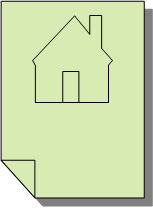
\includegraphics[width=0.25\textwidth]{figures/Homepage-icon.png}
  \end{center}
  \caption{Homepage icon}
  \label{fig:homepageicon}
\end{figure}

\begin{table}[!ht]
  \begin{center}
    \caption{Configurations tested}
    \label{tab:configstested}
    \begin{tabular}{l|c} % <-- Alignments: 1st column left, 2nd middle and 3rd right, with vertical lines in between
      \textbf{Configuration} & \textbf{Description} \\
      \hline
      1 & Simple test with one server\\
      2 & Simple test with one server\\
    \end{tabular}
  \end{center}
\end{table}

\section{Implementation …/Modeling/Simulation/…}

\subsection{Some examples of coding}

Listing~\ref{lst:helloWorldInC} shows an example of a simple program written
in C code.

\begin{lstlisting}[language={C}, caption={Hello world in C code}, label=lst:helloWorldInC]
int main() {
printf("hello, world");
return 0;
}
\end{lstlisting}


In contrast, Listing~\ref{lst:programmes} is an example of code in Python to
get a list of all of the programs at KTH.

\lstset{extendedchars=true}
\begin{lstlisting}[language={Python}, caption={Using a Python program to
    access the KTH API to get all of the programs at KTH}, label=lst:programmes]
KOPPSbaseUrl = 'https://www.kth.se'

def v1_get_programmes():
    global Verbose_Flag
    #
    # Use the KOPPS API to get the data
    # note that this returns XML
    url = "{0}/api/kopps/v1/programme".format(KOPPSbaseUrl)
    if Verbose_Flag:
        print("url: " + url)
    #
    r = requests.get(url)
    if Verbose_Flag:
        print("result of getting v1 programme: {}".format(r.text))
    #
    if r.status_code == requests.codes.ok:
        return r.text           # simply return the XML
    #
    return None
\end{lstlisting}


\cleardoublepage
\chapter{Results and Analysis}
\label{ch:resultsAndAnalysis}
\todo[inline, backgroundcolor=kth-lightblue]{Resultat och analys}

\todo[inline]{
Sometimes this is split into two chapters.\\
  
Keep in mind: How you are going to evaluate what you have done? What are your metrics?\\
Analysis of your data and proposed solution\\
Does this meet the goals which you had when you started?
}

In this chapter, we present the results and discuss them.

\section{Major results}
\todo[inline, backgroundcolor=kth-lightblue]{Huvudsakliga resultat}

Some statistics of the delay measurements are shown in Table~\ref{tab:delayMeasurements}.
The delay has been computed from the time the GET request is received until the response is sent.


\begin{table}[!ht]
  \begin{center}
    \caption{Delay measurement statistics}
    \label{tab:delayMeasurements}
    \begin{tabular}{l|S[table-format=4.2]|S[table-format=3.2]} % <-- Alignments: 1st column left, 2nd middle and 3rd right, with vertical lines in between
      \textbf{Configuration} & \textbf{Average delay (ns)} & \textbf{Median delay (ns)}\\
      \hline
      1 & 467.35 & 450.10\\
      2 & 1687.5 & 901.23\\
    \end{tabular}
  \end{center}
\end{table}

Figure \ref{fig:processing_vs_payload_length} shows and example of the
performance as measured in the experiments.

\begin{figure}[!ht]
% GNUPLOT: LaTeX picture
\setlength{\unitlength}{0.240900pt}
\ifx\plotpoint\undefined\newsavebox{\plotpoint}\fi
\begin{picture}(1500,900)(0,0)
\sbox{\plotpoint}{\rule[-0.200pt]{0.400pt}{0.400pt}}%
\put(171.0,131.0){\rule[-0.200pt]{4.818pt}{0.400pt}}
\put(151,131){\makebox(0,0)[r]{ 1.5}}
\put(1419.0,131.0){\rule[-0.200pt]{4.818pt}{0.400pt}}
\put(171.0,212.0){\rule[-0.200pt]{4.818pt}{0.400pt}}
\put(151,212){\makebox(0,0)[r]{ 2}}
\put(1419.0,212.0){\rule[-0.200pt]{4.818pt}{0.400pt}}
\put(171.0,292.0){\rule[-0.200pt]{4.818pt}{0.400pt}}
\put(151,292){\makebox(0,0)[r]{ 2.5}}
\put(1419.0,292.0){\rule[-0.200pt]{4.818pt}{0.400pt}}
\put(171.0,373.0){\rule[-0.200pt]{4.818pt}{0.400pt}}
\put(151,373){\makebox(0,0)[r]{ 3}}
\put(1419.0,373.0){\rule[-0.200pt]{4.818pt}{0.400pt}}
\put(171.0,454.0){\rule[-0.200pt]{4.818pt}{0.400pt}}
\put(151,454){\makebox(0,0)[r]{ 3.5}}
\put(1419.0,454.0){\rule[-0.200pt]{4.818pt}{0.400pt}}
\put(171.0,534.0){\rule[-0.200pt]{4.818pt}{0.400pt}}
\put(151,534){\makebox(0,0)[r]{ 4}}
\put(1419.0,534.0){\rule[-0.200pt]{4.818pt}{0.400pt}}
\put(171.0,615.0){\rule[-0.200pt]{4.818pt}{0.400pt}}
\put(151,615){\makebox(0,0)[r]{ 4.5}}
\put(1419.0,615.0){\rule[-0.200pt]{4.818pt}{0.400pt}}
\put(171.0,695.0){\rule[-0.200pt]{4.818pt}{0.400pt}}
\put(151,695){\makebox(0,0)[r]{ 5}}
\put(1419.0,695.0){\rule[-0.200pt]{4.818pt}{0.400pt}}
\put(171.0,776.0){\rule[-0.200pt]{4.818pt}{0.400pt}}
\put(151,776){\makebox(0,0)[r]{ 5.5}}
\put(1419.0,776.0){\rule[-0.200pt]{4.818pt}{0.400pt}}
\put(171.0,131.0){\rule[-0.200pt]{0.400pt}{4.818pt}}
\put(171,90){\makebox(0,0){ 0}}
\put(171.0,756.0){\rule[-0.200pt]{0.400pt}{4.818pt}}
\put(298.0,131.0){\rule[-0.200pt]{0.400pt}{4.818pt}}
\put(298,90){\makebox(0,0){ 10}}
\put(298.0,756.0){\rule[-0.200pt]{0.400pt}{4.818pt}}
\put(425.0,131.0){\rule[-0.200pt]{0.400pt}{4.818pt}}
\put(425,90){\makebox(0,0){ 20}}
\put(425.0,756.0){\rule[-0.200pt]{0.400pt}{4.818pt}}
\put(551.0,131.0){\rule[-0.200pt]{0.400pt}{4.818pt}}
\put(551,90){\makebox(0,0){ 30}}
\put(551.0,756.0){\rule[-0.200pt]{0.400pt}{4.818pt}}
\put(678.0,131.0){\rule[-0.200pt]{0.400pt}{4.818pt}}
\put(678,90){\makebox(0,0){ 40}}
\put(678.0,756.0){\rule[-0.200pt]{0.400pt}{4.818pt}}
\put(805.0,131.0){\rule[-0.200pt]{0.400pt}{4.818pt}}
\put(805,90){\makebox(0,0){ 50}}
\put(805.0,756.0){\rule[-0.200pt]{0.400pt}{4.818pt}}
\put(932.0,131.0){\rule[-0.200pt]{0.400pt}{4.818pt}}
\put(932,90){\makebox(0,0){ 60}}
\put(932.0,756.0){\rule[-0.200pt]{0.400pt}{4.818pt}}
\put(1059.0,131.0){\rule[-0.200pt]{0.400pt}{4.818pt}}
\put(1059,90){\makebox(0,0){ 70}}
\put(1059.0,756.0){\rule[-0.200pt]{0.400pt}{4.818pt}}
\put(1185.0,131.0){\rule[-0.200pt]{0.400pt}{4.818pt}}
\put(1185,90){\makebox(0,0){ 80}}
\put(1185.0,756.0){\rule[-0.200pt]{0.400pt}{4.818pt}}
\put(1312.0,131.0){\rule[-0.200pt]{0.400pt}{4.818pt}}
\put(1312,90){\makebox(0,0){ 90}}
\put(1312.0,756.0){\rule[-0.200pt]{0.400pt}{4.818pt}}
\put(1439.0,131.0){\rule[-0.200pt]{0.400pt}{4.818pt}}
\put(1439,90){\makebox(0,0){ 100}}
\put(1439.0,756.0){\rule[-0.200pt]{0.400pt}{4.818pt}}
\put(171.0,131.0){\rule[-0.200pt]{0.400pt}{155.380pt}}
\put(171.0,131.0){\rule[-0.200pt]{305.461pt}{0.400pt}}
\put(1439.0,131.0){\rule[-0.200pt]{0.400pt}{155.380pt}}
\put(171.0,776.0){\rule[-0.200pt]{305.461pt}{0.400pt}}
\put(30,453){\rotatebox{-270}{\makebox(0,0){Processing time (ms)}}}
\put(805,29){\makebox(0,0){Payload size (bytes)}}
\put(868.0,131.0){\rule[-0.200pt]{0.400pt}{84.074pt}}
\put(995.0,131.0){\rule[-0.200pt]{0.400pt}{98.287pt}}
\put(1173.0,131.0){\rule[-0.200pt]{0.400pt}{118.041pt}}
\put(1325.0,131.0){\rule[-0.200pt]{0.400pt}{134.904pt}}
\put(1350.0,131.0){\rule[-0.200pt]{0.400pt}{137.795pt}}
\put(1439.0,131.0){\rule[-0.200pt]{0.400pt}{155.380pt}}
\end{picture}
\caption[A GNUplot figure]{Processing time vs. payload length}\vspace{0.5cm}
\label{fig:processing_vs_payload_length}
\end{figure}
		

Given these measurements, we can calculate our processing bit rate as the inverse of the time it takes to process an additional byte divided by 8 bits per byte:

\[
	bitrate = \frac{1}{\frac{time_{byte}}{8}} = 20.03 \quad kb/s
\] 

\section{Reliability Analysis}
\todo[inline, backgroundcolor=kth-lightblue]{Analys av reliabilitet}

\section{Validity Analysis}
\todo[inline, backgroundcolor=kth-lightblue]{Analys av validitet}


\cleardoublepage
\chapter{Discussion}
\label{ch:discussion}
\todo[inline, backgroundcolor=kth-lightblue]{Diskussion}



\cleardoublepage
\chapter{Conclusions and Future work}
\label{ch:conclusionsAndFutureWork}
\todo[inline, backgroundcolor=kth-lightblue]{Slutsatser och framtida arbete}

\todo[inline]{Add text to introduce the subsections of this chapter.}

\section{Conclusions}
\label{sec:conclusions}
\todo[inline, backgroundcolor=kth-lightblue]{Slutsatser}
\todo[inline]{Describe the conclusions (reflect on the whole introduction given in Chapter 1).}


  
\todo[inline]{Discuss the positive effects and the drawbacks.\\
Describe the evaluation of the results of the degree project.\\
Did you meet your goals?\\
What insights have you gained?\\
What suggestions can you give to others working in this area?\\
If you had it to do again, what would you have done differently?}

\section{Limitations}
\label{sec:limitations}
\todo[inline, backgroundcolor=kth-lightblue]{Begränsande faktorer}
\todo[inline]{What did you find that limited your
  efforts? What are the limitations of your results?}



\section{Future work}
\label{sec:futureWork}
\todo[inline, backgroundcolor=kth-lightblue]{Framtida arbete}
\todo[inline]{Describe valid future work that you or someone else could or should do.\\
Consider: What you have left undone? What are the next obvious things to be done? What hints can you give to the next person who is going to follow up on your work?
}



Due to the breadth of the problem, only some of the initial goals have been
met. In these section we will focus on some of the remaining issues that
should be addressed in future work. ...

\subsection{What has been left undone?}
\label{what-has-been-left-undone}

The prototype does not address the third requirement, \ie, a yearly
unavailability of less than 3 minutes, this remains an open problem. ...

\subsubsection{Cost analysis}

The current prototype works, but the performance from a cost perspective makes
this an impractical solution. Future work must reduce the cost of this
solution, to do so a cost analysis needs to first be done. ...

\subsubsection{Security}

A future research effort is needed to address the security holes that results
from using a self-signed certificate. Page filling text mass. Page filling
text mass. ...


\subsection{Next obvious things to be done}

In particular, the author of this thesis wishes to point out xxxxxx remains as
a problem to be solved. Solving this problem is the next thing that should be
done. ...

\section{Reflections}
\label{sec:reflections}
\todo[inline, backgroundcolor=kth-lightblue]{Reflektioner}
\todo[inline]{What are the relevant economic, social,
  environmental, and ethical aspects of your work?
}




One of the most important results is the reduction in the amount of
energy required to process each packet while at the same time reducing the
time required to process each packet.

The thesis contributes to the \gls{UN}\enspace\glspl{SDG} numbers 1 and 9 by
xxxx. 




\noindent\rule{\textwidth}{0.4mm}
\todo[inline]{In the references, let Zotero or other tool fill this
  in for you. I suggest an extended version of the IEEE  style, to include
  URLs, DOIs, ISBNs, \etc, to make it easier for your reader to find
  them. This will make life easier for your opponents and examiners. \\

  IEEE Editorial Style Manual: \url{https://www.ieee.org/content/dam/ieee-org/ieee/web/org/conferences/style_references_manual.pdf}
}

\cleardoublepage
% Print the bibliography (and make it appear in the table of contents)

\renewcommand{\bibname}{References}
\addcontentsline{toc}{chapter}{References}

\ifbiblatex
    \printbibliography[heading=bibintoc]
\else
    \bibliography{references}
\fi

\cleardoublepage
\appendix
\renewcommand{\chaptermark}[1]{\markboth{Appendix \thechapter\relax:\thinspace\relax#1}{}}
\chapter{Something Extra}
\todo[inline, backgroundcolor=kth-lightblue]{Bilaga}

\section{Just for testing KTH colors}
\ifdigitaloutput
    \textbf{You have selected to optimize for digital output}
\else
    \textbf{You have selected to optimize for print output}
\fi
\begin{itemize}[noitemsep]
    \item Primary color
    \begin{itemize}
    \item \textcolor{kth-blue}{kth-blue \ifdigitaloutput
    actually Deep sea
    \fi} {\color{kth-blue} \rule{0.3\linewidth}{1mm} }\\

    \item \textcolor{kth-blue80}{kth-blue80} {\color{kth-blue80} \rule{0.3\linewidth}{1mm} }\\
\end{itemize}

\item  Secondary colors
\begin{itemize}[noitemsep]
    \item \textcolor{kth-lightblue}{kth-lightblue \ifdigitaloutput
    actually Stratosphere
    \fi} {\color{kth-lightblue} \rule{0.3\linewidth}{1mm} }\\

    \item \textcolor{kth-lightred}{kth-lightred \ifdigitaloutput
    actually Fluorescence\fi} {\color{kth-lightred} \rule{0.3\linewidth}{1mm} }\\

    \item \textcolor{kth-lightred80}{kth-lightred80} {\color{kth-lightred80} \rule{0.3\linewidth}{1mm} }\\

    \item \textcolor{kth-lightgreen}{kth-lightgreen \ifdigitaloutput
    actually Front-lawn\fi} {\color{kth-lightgreen} \rule{0.3\linewidth}{1mm} }\\

    \item \textcolor{kth-coolgray}{kth-coolgray \ifdigitaloutput
    actually Office\fi} {\color{kth-coolgray} \rule{0.3\linewidth}{1mm} }\\

    \item \textcolor{kth-coolgray80}{kth-coolgray80} {\color{kth-coolgray80} \rule{0.3\linewidth}{1mm} }
\end{itemize}
\end{itemize}

\textcolor{black}{black} {\color{black} \rule{\linewidth}{1mm} }
\cleardoublepage
\fancyhead{}  % Do not use header on the following pages
% as the separator pages do not have page numbers or headings and
%the individual included papers will have their own page headings
\chapter{Included papers} % just for some experiments with kthpaper package

\paper{Title of paper}{citation for published or submitted paper}{permission or copyright information}

\paper{A New Automated Way to Measure Polyethylene Wear in THA Using a High Resolution CT Scanner: Method and Analysis}{G. Q. Maguire Jr., M. E. Noz, H. Olivecrona, M. P. Zeleznik, and L. Weidenhielm, “A New Automated Way to Measure Polyethylene Wear in THA Using a High Resolution CT Scanner: Method and Analysis,” \textit{The Scientific World Journal}, vol. 2014, pp. 1–9, 2014. doi: 10.1155/2014/528407.}{Copyright © 2014 Gerald Q. Maguire Jr. \etal. This is an open access article distributed under the \href{http://creativecommons.org/licenses/by/3.0/}{Creative Commons Attribution License}, which permits unrestricted use, distribution, and reproduction in any medium, provided the original work is properly cited.}
\cleardoublepage
\includepdf[pages=-,pagecommand=\thispagestyle{plain}]{./papers/automated_2014-528407.pdf}

\paper{Yet another title}{Oscar Student and A. B. Normal, “Yet another title,” \textit{A Fictitious Journal}, vol. 2021, pp. 1024-2048, 2021. doi: 10.123456789/foo.2021.xxx.}{Copyright © 2021 XXXX. Reprinted with permission.}

\label{pg:lastPageofMainmatter}

\clearpage
\fancyhead{}  % Do not use header on this extra page or pages
\section*{For DIVA}
\divainfo{pg:lastPageofPreface}{pg:lastPageofMainmatter}
\end{document}
